\documentclass[a4paper,11pt,twoside]{report}

\usepackage{color}
\usepackage{listings}
\definecolor{javared}{rgb}{0.6,0,0} % for strings
\definecolor{javagreen}{rgb}{0.25,0.5,0.35} % comments
\definecolor{javapurple}{rgb}{0.5,0,0.35} % keywords
\definecolor{javadocblue}{rgb}{0.25,0.35,0.75} % javadoc
% "define" Scala similar to http://tihlde.org/~eivindw/latex-listings-for-scala/
\lstdefinelanguage{Scala}{
  morekeywords={abstract,case,catch,class,def,%
    do,else,extends,false,final,finally,%
    for,if,implicit,import,match,mixin,%
    new,null,object,override,package,%
    private,protected,requires,return,sealed,%
    super,this,throw,trait,true,try,%
    type,val,var,while,with,yield},
  otherkeywords={=>,<-,<\%,<:,>:,\#},
  sensitive=true,
  morecomment=[l]{//},
  morecomment=[s][\color{javadocblue}]{/**}{*/},
  morestring=[b]",
  morestring=[b]',
  morestring=[b]"""
}
\lstset{
	language=Java,
	keywordstyle=\color{javapurple}\bfseries,
	stringstyle=\color{javared},
	commentstyle=\color{javagreen},
	morecomment=[s][\color{javadocblue}]{/**}{*/},
	numbers=left,
	numberstyle=\tiny\color{black},
	showspaces=false,
	showstringspaces=false,
	breaklines=true,
	tabsize=2
}

\usepackage{fancyhdr}
\pagestyle{fancy}
\cfoot{}
\fancyfoot[LE,RO]{\thepage}

\fancypagestyle{plain}{%
\fancyhf{} % clear all header and footer fields
\fancyfoot[LE,RO]{\bfseries \thepage}
\renewcommand{\headrulewidth}{0pt}}
\setlength{\headheight}{14pt}

%\usepackage{xltxtra}
\usepackage{fontspec}
\setromanfont{Linux Biolinum O}
% \setsansfont[Mapping=tex-text]{DejaVu Sans}
% \setmonofont[Mapping=tex-text]{DejaVu Sans Mono}

\usepackage{url}

\usepackage[footnote]{acronym}
\acrodef{API}{Application Programming Interface}
\acrodef{FAQ}{Frequently Asked Question}
\acrodef{ICU}{International Components for Unicode}
\acrodef{ISO}{International Organization for Standardization}
\acrodef{JAR}{Java Archive}
\acrodef{JSON}{JavaScript Object Notation}
\acrodef{PO}{Portable Object}
\acrodef{UI}{User Interface}
\acrodef{USA}{United States of America}

\usepackage{varioref}

\usepackage[style=numeric, backend=biber, sorting=none]{biblatex}
\bibliography{references.bib}
\DeclareFieldFormat{url}{\newline\url{#1}}

\usepackage[bookmarks=true]{hyperref}
\hypersetup{
    pdftitle={translatables User Documentation},    % title
    pdfauthor={Augustus Kling},                     % author
    pdfsubject={translatables},                        % subject of the document
    pdfkeywords={translatables, localization, translation}, % list of keywords
    colorlinks=true,       % false: boxed links; true: colored links
    linkcolor=blue,       % color of internal links
    citecolor=black,       % color of links to bibliography
    filecolor=black,        % color of file links
    urlcolor=blue,        % color of external links
    linktoc=all            % only page is linked
}%

\usepackage{parskip}
\setlength{\parindent}{17pt}

\title{Introduction to Localization And Manual for translatables}
\author{Augustus Kling}
\date{\today}

\begin{document}
\maketitle

\tableofcontents

\chapter{Localization in General}
Localization is the process of modifying a software so that it can be used in multiple languages. This allows an international user group to actually make use of the software because its user interface begins to speak the user's language and uses familiar conventions for formatting, too. The concepts explained in this document can only be sensibly applied when translating many small texts (such as a \ac{UI}) and don't help with the translation of large documents.

Technically, localization includes wrapping texts that need translations in method calls to allow for substitution. The substitution will then provide the desired text based on the target language and possibly placeholder values. A step by step introduction can be found in the Java Tutorials \cite{java-i18n-intro}.

In the simplest case substitution means to look up the translation from the text as appearing in the source code. However this requires extra code branches to select proper messages because grammar and especially pluralization differs vastly across languages. Not only is the process tedious, the readability of the code is impeded due to the increased amount of code. Translating this way is impractical as the programmer would need to know the target languages' grammar\footnote{Grammar for pluralization alone a highly complex task \cite{unicode-plural-remarks} as a language comparison \cite{unicode-plural-rules} shows.}.

There are various libraries that try to aid in development by extracting translations, choosing correct translations and possibly help with formatting of values, too. Sadly, value formatting requires explicit calls with most libraries and pluralization gets difficult as some languages mutate the sentence dependent on placeholder values.

\section{Commonly Used Software}
Available tools range from basically doing everything in own code to pretty much automated solutions. The former fails to provide good results due to the required complexity when things need to be right. The latter is promising but often requires to extract translations manually or requires the the programmer to format placeholders.
\begin{description}
	\item[ICU] \ac{ICU} is developed in C++ but offering a Java binding. No automated extraction. Handles most cases in about any language.
	\item[gettext] Bindings are available for most programming languages and so are mature tools. Placeholder formatting is left to the programmer and pluralization needs to be handled explicitly, though not manually. The translator has to understand the text formatting functions and those differ across programming languages where gettext is available.
	\item[Java native] Manual key extraction and pluralization not handled automatically.
\end{description}
Make sure to choose a tool that automates as much as possible as this gets the error rates down. Automatic key extraction is a must-have feature and pluralization can only be neglected when it is absolutely sure that the set of target languages never changes. One should also value common data formats for the translations.

You should check out gettext and its tool ecosystem unless you have already decided on the tools to use. Note that translatables is able to work with gettext's \ac{PO} file format which can be used by most desktop software for translators.

\section{Challenges}
One should provide software that adapts to the users language to facilitate use of the software. Additionally, most users feel more comfortable working in their mother tongue than in a foreign language. This requires that software development takes languages into account. Not only does this need development time but can lead to dissatisfaction if not done right. Half-baked localization makes software hard to use and can even result in misconceived data.

It is not feasible to handle translations manually because acceptable quality cannot be reached this way with reasonable cost. Programmers cannot be expected to be fluent in many natural languages and translators cannot be expected to be able to work with source code so an intermediate layer is required to allow each profession completing their localization task. One needs a tool that handles extraction of translatable text from source code, grammar and pluralization and possibly formatting of values such as dates, times and numbers.

\chapter{translatables}
The following terms are use throughout the documentation for describing concepts precisely. While details are not important to get started with translatables, it helps to grasp the workings behind the surface.
\begin{description}
	\item[Source Key] Text to be translated as it appears in the source code. A source key can refer to multiple translations of which one is chosen as soon as values for all placeholders are known. Source keys are language agnostic.
	\item[Translation Key] Identifier of a translation. Those are automatically generated from the source keys in dependence of placeholder types. The amount of translation keys varies across languages where more complex grammar usually means more translation keys.
	\item[Domain] Type of a placeholder. All languages support plain text, numbers, gender, date, time and currencies. Domains define the formatting of values and user-defined types can be added if required.
	\item[Category] Values are examined and grouped according to the grammar of the target language in a way that the same grammar applies for all values in a category. For example if a target language has 3 plural forms, 3 categories would result for the number domain.
\end{description}
\section{Core Concept}
translatables tries to abstract most of the localization process so that your code stays as clean as possible – that is as unaffected as possible. To do so static messages are simply looked up while values with placeholders are looked up after determining their lookup key (translation key) based on the runtime values of all placeholders. Once a translation was found it is filled with placeholder values like they are expected to be formatted given the target language and region.

Suppose we wanted to inform about executed transactions with a translated message to illustrate the translation process with an example.
\begin{quotation}
Executed \{number(0)\} transactions
\end{quotation}
Note that \verb|0| is a placeholder name that takes a number and one would call it like \lstinline$System.out.println(tr("Executed {number(0)} transactions", a))$. Assuming you are translating to French and the variable \verb|a| is 1815, translatables would determine the pluralization rule\footnote{French has 2 plural forms. A form for the number 0 or 1, and another for all other numbers. Compare this with English where 2 forms exist for either 1 or all other numbers.} for everything bigger than one and try to look up the translation for \textit{Executed \{number(two(0))\} transactions}. Afterwards it would format the value 1815 to get \textit{1\,815}\footnote{Blocks of three digits are separated with thin spaces.} and insert this into the translated text to get something like \textit{Exécuté 1\,815 transactions}.

Your application code was not cluttered with additional branches and the programmer only had to state that a number was to be inserted. It was not necessary to have a programmer that is familiar with French pluralization rules and the translator got a simple example sentence which allowed to get the grammar exactly right without any programming knowledge.

In general each application provides an own translation call, \lstinline$tr$ in the example above, to implement the language selection and loading of translations because the translatables library cannot know if you are depending on system locales or allow the user to choose a language. The requirement to load translations yourself exists to keep the library format agnostic. A typical implementation of a translation call is a few lines of code as shown in the code samples below.

\subsection{Identifying Translations}
Most translation systems rely on invented keys to identify translations but translatables makes use of natural language sources in combination with domains. Even though one is not constrained to use natural language to identify translations, it simplifies the translation process.

In practice the programmer types in the source key (which could be an English sentence or an invented key) and marks the translation with a method call and leaves the rest to translatables' automatisms. Usage of natural languages is shown in the usage examples.

\subsection{Placeholders}
At times messages require translations that contain dynamic parts. Think about including a person's name or a calculated number as examples.

Placeholders are typed right into the source keys by the programmer and can optionally be bound to a value domain if special treatment is desired. Values that don't require special treatment are plain text. Treatment is required for numbers (plural forms), dates (formatting rules) and other domains and is handled by translatables according to the grammar of the target language and the conventions of the targeted region.

The code examples do only show numeric placeholder names as those are the most convenient to work with but named placeholders can be used as well. Named placeholders are useful in the rare event of messages with lots of placeholders in them or for added clarity. Placeholders are always given enclosed in brackets and will be replaced at runtime including brackets.

\begin{description}
	\item[\{2\}] Third numeric placeholder. Note that the number only serves to identify the placeholder and does not restrict the values to be inserted nor the order in which the placeholders appear. The \textit{plain} domain will be used and the placeholder value will be inserted unchanged because no domain was explicitly given.
	\item[\{testname\}] Semantically equal to numeric placeholders but the names can make it easier for programmers and translators to grasp the meaning of the inserted value.
	\item[\{number(0)\}] First numeric placeholder that is bound to the \textit{number} domain. Translatables will automatically generate translation keys according to the pluralization rules of the target language. The correct translation will be chosen at runtime when the placeholder's value is known.
	\item[\{number(testname)\}] Semantically equal to numeric placeholder for \textit{number} domain.
\end{description}

Any number of placeholders can be used in a message and domains are specified per placeholder. A mix of numeric and named placeholder can be used in the same message. In fact the numeric placeholders are just using digits as variable names – they don't have special semantics.

\section{Usage Examples}
For both, Scala and Java, either a method call or an annotation serves as marker for translatable texts. Those texts can be extracted automatically by translatables and actually be translated at runtime by invoking a translation method as shown in detail in section \vref{sec:library-binding} when translatables \ac{API} is discussed.

Please note that the name of the translation method can be chosen when invoking the translation extraction. What matters is, that the method takes a string literal as its first parameter – a string variable won't work as its value is only known at runtime and not available during extraction.

\begin{lstlisting}[caption=Methods as markers]
import static your.application.tr;

public class Test {
	public static void main(String[] args){
		String translatedValue1 = tr("This is a sample");
		String translatedValue2
		 = tr("You've received {number(0)} messages.", 8);
	}
}
\end{lstlisting}

\begin{lstlisting}[caption=Annotations as markers]
import static your.application.tr;

public class Test {
	@TranslationKey
	final String yourSourceKey = "This is a sample";
	
	@TranslationKey
	final String yourSourceKey2
	 = "You've received {number(0)} messages.";
	
	public static void main(String[] args){
		String translatedValue1 = tr(yourSourceKey);
		String translatedValue2 = tr(yourSourceKey2, 8);
	}
}
\end{lstlisting}

The \lstinline$TranslationKey$ annotation serves as marker for a field only. It does not lead to any translation of the value. Ensure to pass such fields to a translation method as shown.

\section{Supported Languages}
translatables aims to support a wide variety of languages and regions and chances are your desired language is supported. Please do request any additional languages required.

When using translatables simply provide a language and country code as shown below in this documentation in the library binding example code.

\section{Binding the Library}\label{sec:library-binding}
translatables is provided as 2 \ac{JAR} files. One variant contains all of its dependencies whilst the alternative is optimized for size and expects your build process to supply the dependencies. In either case you should implement the translation method as shown in the sample codes for Scala (section \vref{sec:scala-translation-function}) or Java (section \vref{sec:java-translation-function}).

\subsection{Eclipse}
Link translatables to your project by setting the project's build path. Do so by clicking your project in the “Project Explorer” and open its properties via the context menu or \textit{File} → \textit{Properties}. Select \textit{Build Path} in the tree.
\begin{figure}
	\centering
	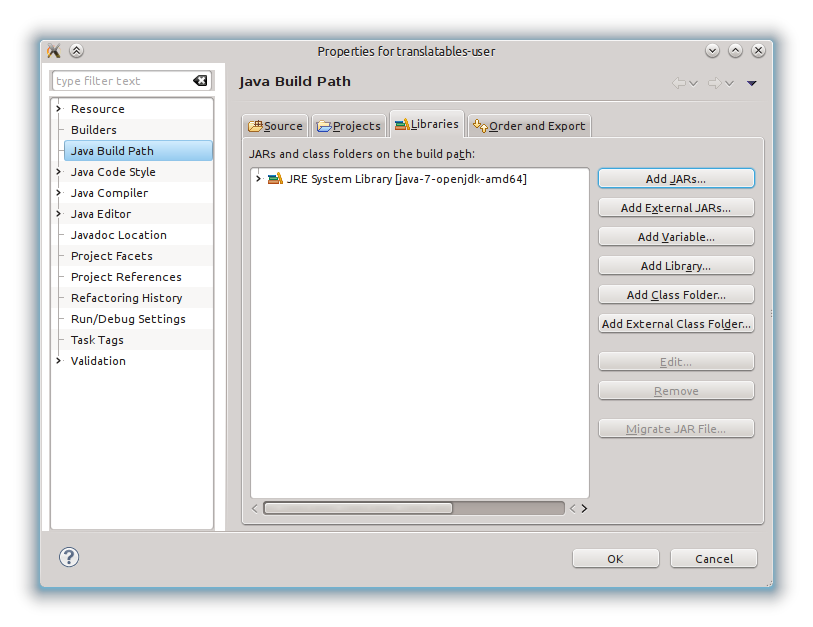
\includegraphics[width=\textwidth]{./images/build-path.png}
	% build-path.png: 0x0 pixel, 300dpi, 0.00x0.00 cm, bb=
	\caption{Build path configuration in Eclipse}
\end{figure}
Press “Add external JARs…” and select the translatables \ac{JAR} file. Choose the full \ac{JAR} so Eclipse will show targeted tooltips and \ac{API} documentation. The linking just made is enough that Eclipse is able to import the required classes and manage\footnote{See \cite{java-class-resolving} for details on how Java resolves classes.} the class path automatically.

\subsection{System Requirements}
\begin{itemize}
	\item Java 7.
	\item Scala library on classpath.\footnote{Does not apply when using the full build as it provides the Scala library.}
\end{itemize}

\subsection{Scala}\label{sec:scala-translation-function}
Define a method that determines the language of the user and provides the location where the translations are stored. The method can then be imported where needed to make convenient use of it.
\begin{lstlisting}[language=Scala]
/**
 * Translates a text, inserts formatted placeholder values.
 * @param key Source key. Might contain placeholders with numeric names.
 * @param placeholder Any number of values to insert.
 * @return Translated text.
 */
 def tr(key:String, placeholder:Object*):String = {
	// TODO Determine lang based on your application's language settings.
	val locale:Locale = Locale.getDefault();
	val lang:Language = Language.fromLocale(locale);

	// TODO Get translations from your infrastructure (for example property file, database).
	val translationFile:File = new File("translations/"
			+ lang.code().getLanguage() + ".json");
	val translations:Adapter = new JsonAdapter(translationFile);
	
	Translation.getVariadic(language, translations, key, placeholders: _*)
 }
\end{lstlisting}
Note that the \lstinline$Translation$ object holds more methods to work with placeholders from lists, maps and tuples which you might find useful, too.

\subsection{Java}\label{sec:java-translation-function}
Place a fragment similar to the listing somewhere in your application where you can access it easily. It's usually most comfortable if you allow for a static import of the translation call. In most cases you want to cache the language and translations within the JVM.
\begin{lstlisting}
/**
 * Translates a text, inserts formatted placeholder values.
 * @param key Source key. Might contain placeholders with numeric names.
 * @param placeholder Any number of values to insert.
 * @return Translated text.
 */
private static String tr(String key, Object... placeholder) {
	// TODO Determine lang based on your application's language settings.
	Locale locale = Locale.getDefault();
	Language lang = Language.fromLocale(locale);

	// TODO Get translations from your infrastructure (for example property file, database).
	File translationFile = new File("translations/"
			+ lang.code().getLanguage() + ".json");
	Adapter translations = new JsonAdapter(translationFile);

	return JavaApi.instance
			.getVariadic(lang, translations, key, placeholder);
}
\end{lstlisting}
The rest of the application simply uses the method and does not bother much about translations:
\begin{lstlisting}
String translated = tr("Hello {0}, it's {time(1)}!",
	"plaintext to insert", new java.util.Date());
\end{lstlisting}

\section{Extracting Translations}
When your application grows it is important to be able to extract translations in an automated manner because it is tedious and error-prone to maintain the translation list manually. The automatic extraction of translations guarantees that the translation list is complete and as short as possible for any target language. It is expected that the number of required translations differs across languages due to the varying complexity of the grammars.

The translatables library\footnote{Variant including dependencies only.} can be run as command line tool for automatic extraction and management of translations. New translations are detected and merged with the existing translations and unused translations are discarded. Run the program without parameters to see the documentation of its parameters. Usually, you want to use a call similar to:
\begin{verbatim}
java -jar translatables.jar extract --source /application/src/
  --target /application/translations/de.json --language de
  --calls tr
\end{verbatim} 
The call instructs translatables to examine all source code recursively which resides in \path{/application/src/}. Translations are generated based on the rules that apply for German and written to \path{/application/translations/de.json}. Furthermore it is assumed that you've called your translation method \lstinline$tr$ as shown in the example code above. Additional sources or translation methods can be given by repeating the parameters.

Numerous languages are supported and can be chosen by specifying their code according to \ac{ISO} 639-1 (two letter codes) and \ac{ISO} 639-2 (three letter codes) where no \ac{ISO} 639-1 code exists. Grammar and placeholder formatting is then automatically handled. Country codes can be given according to \ac{ISO} 3166 (Alpha-2 code) to further specialize the underlying rules. Thus \textit{pt\_BR} would mean Portuguese as spoken in Brazil.

It is recommended to invoke the extraction from a build script so that translations for all desired languages can be updated easily. Translations can be stored in \ac{JSON}, Java-properties or \ac{PO} files but see \vref{formats} for details.

\section{Supplying Translations}
Once translations have been extracted the empty translation files can be passed to a translator. Simply translating all example sentences will be sufficient and there is no need for the translator to access the source code of the application to be translated.

Suppose the extraction emitted the following file for passing on to a translator.
\begin{lstlisting}
{
	"Executed {number(zero(0))} transactions": "",
	"Executed {number(one(0))} transactions": ""
}
\end{lstlisting}

The translator would look for empty translations with a simple text editor or using a sophisticated translation environment and fill in the blanks. Afterwards the translator sends back a file similar to the following which is to be used instead of the automatically generated file.
\begin{lstlisting}
{
	"Executed {number(zero(0))} transactions": "{0} Transaktionen wurden ausgeführt",
	"Executed {number(one(0))} transactions": "{0} Transaktion wurde ausgeführt"
}
\end{lstlisting}
The placeholders are given in brackets and obviously a repetition of value domains (types) is not necessary. In case the translator wanted to display brackets as part of the translation they are to be duplicated. Upon receiving the augmented file there is nothing more to do for the programmer than to copy it over the automatically generated file.

Thus adding new languages means invoking the automatic extraction, sending the generated file and copying over the augmented file. It is not necessary to even touch an application's code in order to make it available in unexpected languages.

\section{Formats}\label{formats}
translatables supports a number of formats among which you should be able to find one that fulfills your needs. Namely, the supported formats are:
\begin{description}
	\item[\ac{JSON}] Simple key to value mappings with libraries available in about any programming language. Common translations tools do seldom support the format.
	\item[Java properties] Key to value mappings. A lot of Java based programs already use this format due to its integration into the Java platform.
	\item[\ac{PO} file] gettext's format which offers support for fuzzy flagging and allows the translators to store comments along with the translations. Very good tool support.
\end{description}

Note that the support for \ac{PO} files just maps the generated translation keys to message identifiers and translations are expected to be always given in gettext's field for singular translations. The reason for this is that translatables supports multiple placeholders per translation in addition to gettext and uses its own placeholder formatting. Those concepts cannot be mapped directly to gettext's concepts. The mapping to purely singular translations in \ac{PO} files does allow to use all features of translatables and most features of the translation tools for \ac{PO} files, too.

\section{Pseudo Translations}
It is useful to be able to assess if all required texts have been translated during development before actual translations are available. Pseudo translations allow this by using modified versions of the source keys as translations. More precisely, a prefix and suffix is added to simulate text expansion in languages that use longer words than your source language. Those additions make it easy to spot forgotten translations, too.

For that encoding of characters turns out to be an issue at times the pseudo translations use characters with randomly added diacritics built from the source keys. Thus the pseudo translations can still be read when testing an application during development but show up as garbled when your application does not handle character encoding properly. For example the pseudo-translation for “new translations” should show up as “ñḕẘ ŧȑáñșłáŧıǫñș”.

Pseudo translations are not useful for the end-user and are supposed to be used during development only.

\section{Additional Examples}
This section aims to showcase some of translatables' features by providing source extracts along with extracted translations and generated output. You may find it helpful as a \ac{FAQ} like example list to copy from.

\subsection{Substitution}
Shows placement of a value in a translation. The translation will be fetched by translatables based on the value of the placeholder.
\begin{lstlisting}
System.out.println(trDoc("Simple."));
System.out.println(trDoc("Hello {0}", "Peter"));
System.out.println(trDoc("Hello {0} and {1}", "Peter", "Anna"));
System.out.println(trDoc("There are {number(0)} outdated data sets.", 8));
\end{lstlisting}
After the translations are extracted using the command line tool we are left with a translation file to fill out.

\begin{verbatim}
java -jar translatables-extractor.jar --source src/
  --target translations-de_DE.json --language de_DE
  --calls trDoc
\end{verbatim}

Doing so gives the following translations.
\begin{lstlisting}[escapechar=\&]
{
	"Hello {plain(0)}" : "Hallo {0}",
	"Hello {plain(0)} and {plain(1)}" : "Hallo {0} und {1}",
	"Simple." : "Einfach.",
	"There are {one(number(0))} outdated data sets." :&\linebreak&"Es gibt {0} veralteten Datensatz.",
	"There are {zero(number(0))} outdated data sets." : "Es gibt {0} veraltete Datensätze."
}
\end{lstlisting}
Running the Java code results in the output of the correct sentences. Note that the sentence with the correct plural form has been picked.
\begin{lstlisting}
Einfach.
Hallo Peter
Hallo Peter und Anna
Es gibt 8 veraltete Datensätze.
\end{lstlisting}

\subsection{Substitution with Formatting}
Some classes of values need to be formatted dependent on the language and region for which texts are emitted. Most notably this affects the decimal separator, ordering of the elements of a date and formatting of times.
\begin{lstlisting}
System.out.println(trDoc("A high number: {number(0)}", 123456789.23456789));
System.out.println(trDoc("Swimming on {date(0)} is enjoyable.", new Date(100,8,2)));
System.out.println(trDoc("Next appointment due today at {time(0)}.", Calendar.getInstance().getTime()));
\end{lstlisting}
Extracting the translations and filling the blanks results in:
\begin{lstlisting}[escapechar=\&]
{
	"A high number: {one(number(0))}" :&\linebreak&"Eine hohe Zahl: {0}",
	"A high number: {zero(number(0))}" :&\linebreak&"Eine hohe Zahl: {0}",
	"Next appointment due today at {local(time(0))}." : "Nächster Termin heute um {0}.",
	"Swimming on {digits(date(0))} is enjoyable." :&\linebreak&"Schwimmen am {0} is angenehm.",
}
\end{lstlisting}
When executed with a German locale bound to Germany and English bound to the \ac{USA} the following outputs result.
\begin{lstlisting}
Eine hohe Zahl: 123.456.789,235
Schwimmen am 02.09.2000 is angenehm.
Nächster Termin heute um 23:31.
\end{lstlisting}

\begin{lstlisting}
A high number: 123,456,789.235
Swimming on Sep 2, 2000 is enjoyable.
Next appointment due today at 11:34 PM.
\end{lstlisting}

\subsection{Formatting Application Data Types}
An application will always define its own data types, most likely classes, to represent domain specific concepts. Depending on what is represented support for those types in translatables is desirable. For the sake of an example suppose your application works with monetary values and uses Joda money. To support embedding such monetary values within translations and have them formatted appropriately by translatables a domain needs to be implemented.
\begin{lstlisting}
// Application data type.
import org.joda.money.Money;

// Built-in domain or translatables.Domain
import domains.Currency;

public class JodaMoneyCurrency extends Currency {

	// Calling super constructor omitted for brevity.

	@Override
	public String format(Object value) {
		// Handle application data type.
		if (value instanceof Money) {
			NumberFormat formatter = NumberFormat
					.getCurrencyInstance(this.locale);
			Money jodaValue = (Money) value;
			formatter.setCurrency(java.util.Currency.getInstance(jodaValue
					.getCurrencyUnit().getCurrencyCode()));
			return formatter.format(jodaValue.getAmount());
		}
		// Handle built-in data types.
		return super.format(value);
	}
}
\end{lstlisting}

In principle the newly created domain will apply its logic when the application specific data type is encountered. Otherwise it simply redirects to the default formatting implementation to handle other data types.

To make translatables aware of the new domain, create a sub class of the Language object to use. One could create a wrapper to prioritize the new domain or implement a class per language.
\begin{lstlisting}
import translatables.Language;

public class WithApplicationDomain extends Language {

	public WithApplicationDomain(Language base) {
		super(base.code(), Arrays.asList(
			new JodaMoneyCurrency(base.code())
		), base);
	}
}
\end{lstlisting}
The example classes can now be used to format Joda money values. Therefore translating to German by calling \lstinline$tr("That's {currency(0)} to pay", Money.of(CurrencyUnit.EUR, 1234.56))$ results in \textit{Das macht 1.234,56 €}.

\section{Feedback}
Please file any issues you might encounter at:
\newline\url{https://github.com/AugustusKling/translatables}.

\printbibliography
\end{document}
